%%%%%%%%%%%%%%%%%%%%%%%%%%%%%%%%%%%%%%%%%%%%%%%%%%%%%%%%%%%%%%%%%%%%%%%%%%%%%%%
%                     Отчёт по лабораторной работе №3
%
% Дисциплина: Теория вероятностей и Математическая статистика
%                     
% Название:   Построение боксплотов Тьюки и оценка выбросов
%
% Выполнил:   Михаил Маляренко
%
% Дата:       24 Ноя. 2020
%
%%%%%%%%%%%%%%%%%%%%%%%%%%%%%%%%%%%%%%%%%%%%%%%%%%%%%%%%%%%%%%%%%%%%%%%%%%%%%%%

% HEADER BEGIN 
\documentclass[12pt]{article}
\usepackage[utf8]{inputenc}
\usepackage[russian]{babel}
\usepackage{pscyr}
\usepackage[T2A]{fontenc}
\usepackage{geometry}
\usepackage{graphicx}
\usepackage{multirow}
\usepackage{amsmath}
\usepackage{amssymb}
\usepackage{hyperref}
\usepackage{xcolor}

\geometry {	
	a4paper, 
	left   = 20mm, 
	right  = 20mm, 
	top    = 20mm, 
	bottom = 20mm
}

\definecolor{urlcolor}{HTML}{2484BC} 
\definecolor{linkcolor}{HTML}{000000}

\graphicspath{{resource/}}
% HEADER END

% DIFINES BEGIN
\newcommand{\lskip}{\hfill\break}
% DEFINES END

\begin{document}

\begin{titlepage}
	\begin{center}
		\hfill \break
		{\textbf{Санкт-Петербургский политехнический университет Петра Великого}}\\
		\hfill \break
		\textbf{Институт прикладной математики и механики}\\
		 \hfill \break
		\textbf{Кафедра <<Телематика (при ЦНИИ РТК)>>}\\
		\vfill
		\large{\bfseries Отчет по лабораторной работе}\\
		\hfill \break
		\hfill \break
		\hfill \break
		\hfill \break
		\normalsize{\bfseries Построение боксплотов Тьюки и оценка выбросов}\\
		По дисциплине <<Теория вероятностей и Математическая статистика>>\\
		\hfill \break
		\hfill \break
		\hfill \break
	\end{center}
 
	\normalsize
	{ 
		\begin{tabular}{lp{2cm}cr}
			Выполнил &&&\\
			Студент гр. 3630201/80101&&\underline{\hspace{1.5cm}}& М.Д. Маляренко\\\\
			Руководитель&&&\\ 
			к.ф.-м.н., доцент && \underline{\hspace{1.5cm}}& А.Н. Баженов \\\\
			&&&<<\underline{\phantom{333}}>>\underline{\phantom{сентября000}}
			2020г.
		\end{tabular}
	}
\vfill

\begin{center} Санкт-Петербург \\2020 \end{center}
\end{titlepage}

\newpage

\setcounter{page}{2}

\begin{flushleft}

\setlength{\parindent}{1cm}

% TABLE OF CONTENTS
\tableofcontents

\newpage

% LIST OF FIGURES
\listoffigures

\newpage

% LIST OF TABLES
\listoftables

\newpage

\section{Постановка задачи}
    
	Заданы 5 распределений случайных величин:

	\begin{enumerate}
		\item Нормальное распределение $N(x, 0, 1)$
		\item Распределение Коши $C(x, 0, 1)$
		\item Распределение Лапласа $L(x, 0, 1/\sqrt{2})$
		\item Дискретное распределение Пуассона $P(k, 10)$
		\item Равномерное распределение $U(x, -\sqrt{3}, \sqrt{3})$
	\end{enumerate}

    \noindentДля каждого распределения необходимо сгенерировать выборки размером в 20, 100 элементов. Для каждой выборки построить боксплот Тьюки.
    
    Сгенерировав каждую выборку 1000 раз и определить среднюю экспериментальную долю выбросов и сравнить её с теоретической вероятностью выбросов $P_{\text{\tiny{B}}}^{\text{\tiny{T}}}$ для рассматриваемого распределения. 

\newpage

\section{Теория}

    \subsection{Боксплот Тьюки}

        Боксплот Тьюки (a.k.a. ящик с усами) -- график, использующийся в описательной статистике, компактно изображающий одномерное распределение вероятностей.\cite{theory}

        Боксплот представляет собой прямоугольник с исходящими из боков отрезками-усами и прямой перпендикулярной усам линией внутри прямоугольника. Боксплот располагается на числовой оси. Левая и правая границы прямоугольника определяют соответственно первую выборочную квартиль $Q_1$ и третью выборочную квартиль $Q_3$, центральная линия указывает положение медианы выборки. Отрезки-усы определяют границы статистически значимой выборки, и вычисляются по следующим формулам:

        \begin{equation}
            X_1 = Q_1 - \frac{3}{2} (Q_3 - Q_1); \qquad X_2 = Q_3 + \frac{3}{2} (Q_3 - Q_1)
            \label{whiskers}
        \end{equation}

        \noindent, где $X_1$ -- нижняя граница усов, $X_2$ -- верхняя граница усов. Элементы выборки, выходящие за границы, определённой усами, называются выбросами и обозначаются небольшими кружками.

    \subsection{Теоретическая вероятность выбросов}

        Найдя по функции распределения теоретические значения первой и третьей квартили $Q_1^{\text{\tiny{T}}}$ и $Q_3^{\text{\tiny{T}}}$, по формуле (\ref{whiskers}) можно вычислить теоретические границы усов $X_1^{\text{\tiny{T}}}$ и $X_2^{\text{\tiny{T}}}$.

        Теоретическая вероятность выбросов вычисляется по формуле:\cite{boxplot}

        \begin{itemize}
            \item Для непрерывных распределений

            \begin{equation}
                P_{\text{\tiny{B}}}^{\text{\tiny{T}}} = P(x < X_1^{\text{\tiny{T}}}) + P(x > X_2^{\text{\tiny{T}}}) = F(X_1^{\text{\tiny{T}}}) + (1 - F(X_2^{\text{\tiny{T}}}))
                \label{PС}
            \end{equation}

            \item Для дискретных распределений
            
            \begin{equation}
                P_{\text{\tiny{B}}}^{\text{\tiny{T}}} = P(x < X_1^{\text{\tiny{T}}}) + P(x > X_2^{\text{\tiny{T}}}) = (F(X_1^{\text{\tiny{T}}}) - P(x = X_1^{\text{\tiny{T}}})) + (1 - F(X_2^{\text{\tiny{T}}}))
                \label{PD}
            \end{equation}
            
        \end{itemize}

        \noindent, где $F(X)$ -- функция распределения.

\newpage

\section{Реализация}

Построение графиков и расчёты теоретической вероятности и экспериментальной доли выбросов производилось в среде аналитических вычислений Maxima. Графики построены с помощью интегрированной утилиты gnuplot. Полный код скрипта для среды Maxima представлен в репозитории GitHub. 

\newpage

\section{Результаты}

    \subsection{Боксплоты Тьюки}

        По полученным выборкам были построены боксплоты Тьюки. На Рис. 1-5 представлены боксплоты выборок из 20 и 100 элементов, соответствующих заданным распределениям.
        
        \begin{figure}[h]
            \center{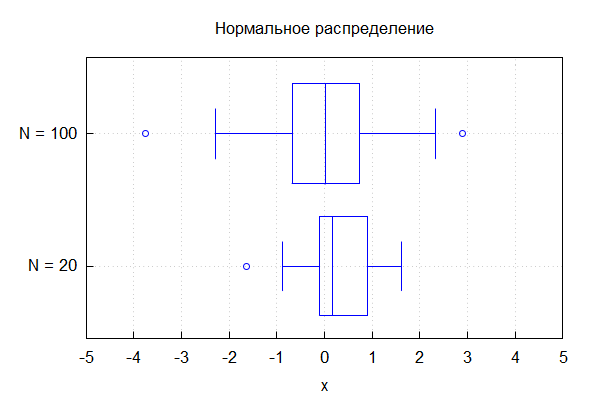
\includegraphics[width=0.75\linewidth]{BP_N.png}}
            \caption{Боксплот выборок нормального распределения}
        \end{figure}

        \begin{figure}[h]
            \center{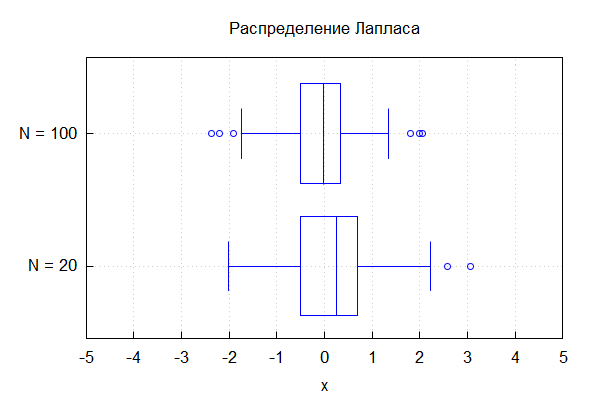
\includegraphics[width=0.75\linewidth]{BP_L.png}}
            \caption{Боксплот выборок распределения Лапласа}
        \end{figure}

        \newpage
        \lskip
        \lskip
        \lskip

        \begin{figure}[h]
            \center{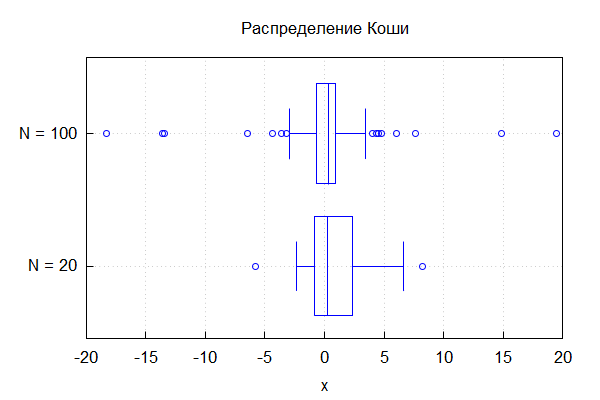
\includegraphics[width=0.75\linewidth]{BP_C.png}}
            \caption{Боксплот выборок распределения Коши}
        \end{figure}

        \begin{figure}[h]
            \center{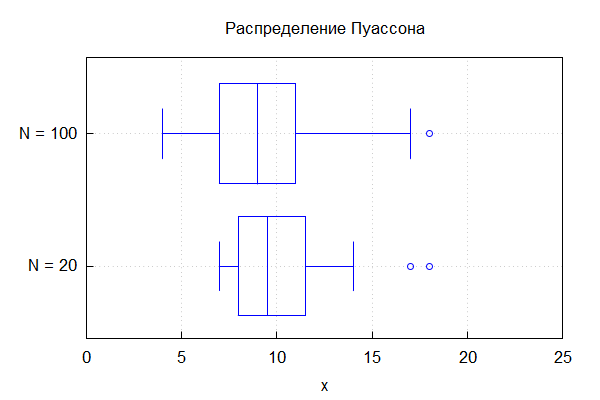
\includegraphics[width=0.75\linewidth]{BP_P.png}}
            \caption{Боксплот выборок распределения Пуассона}
        \end{figure}

        \newpage

        \begin{figure}[h]
            \center{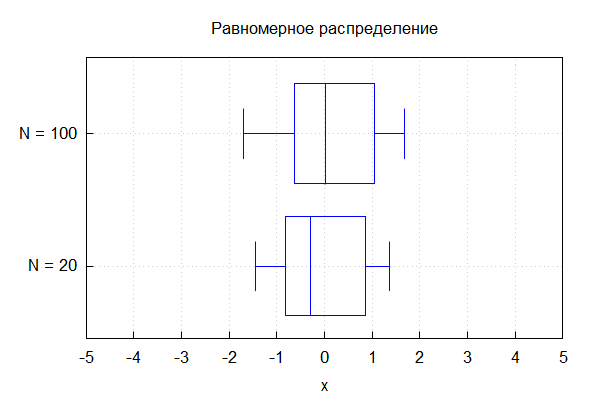
\includegraphics[width=0.75\linewidth]{BP_U.png}}
            \caption{Боксплот выборок равномерного распределения}
        \end{figure}

    \subsection{Сравнение теоретической вероятности и экспериментальной доли выбросов}

        Для 1000 экземпляров каждой выборки была вычислена средняя доля выбросов. Теоритическая вероятность выброса $P_{\text{\tiny{B}}}^{\text{\tiny{T}}}$ рассчитана по формуле (\ref{PС}). 
        \lskip

        \noindentПогрешность средней доли выброса рассчитана следующим образом
        \begin{equation}
            \Delta_z = \sqrt{\left(\overline{z^2} - {\overline{z}}^2\right)}
            \label{delta}
        \end{equation}

        \noindentЗначение экспериментальной доли выброса округлено согласно погрешности. Результаты вычислений представлены в Таблице 1.

        \begin{table}[h]
            \begin{center}
                \begin{tabular}{|*{4}{c|}}\hline
                    \multirow{2}*{Распределение}  & \multirow{2}*{$N$} & Доля & \multirow{2}*{$P_{\text{\tiny{B}}}^{\text{\tiny{T}}}$} \\
                    & & выбросов & \\ \hline \hline
                    \multirow{2}*{Нормальное} & $20$ & $0.00 \pm 0.02$\;(\ref{delta}) & \multirow{2}*{$0.0069$} \\ \cline{2-3}
                    & $100$ & $0.007 \pm 0.009$ & \\ \hline
                    \multirow{2}*{Лапласа} & $20$ & $0.06 \pm 0.06$ & \multirow{2}*{$0.0625$} \\ \cline{2-3}
                    & $100$ & $0.06 \pm 0.03$ & \\ \hline
                    \multirow{2}*{Коши} & $20$ & $0.16 \pm 0.08$ & \multirow{2}*{$0.156$} \\ \cline{2-3}
                    & $100$ & $0.16 \pm 0.04$ & \\ \hline
                    \multirow{2}*{Пуассона} & $20$ & $0.01 \pm 0.02$ & \multirow{2}*{$0.0099$} \\ \cline{2-3}
                    & $100$ & $0.007 \pm 0.009$ & \\ \hline
                    \multirow{2}*{Равномерное} & $20$ & $0.0 \pm 0.0$ & \multirow{2}*{$0.0$} \\ \cline{2-3}
                    & $100$ & $0.0 \pm 0.0$ & \\ \hline
                \end{tabular}
            \caption{Сравнение экспериментальной доли и теоретической вероятности выбросов}
            \end{center}
        \end{table}

\newpage

\section*{Заключение}
\addcontentsline{toc}{section}{Заключение}

В результате лабораторной работы были построены боксплоты Тьюки по выборкам, согласно пяти заданным распределениям. По ним визуально были оценены мощности выбросов распределений.

Также была рассчитана теоретическая вероятность выбросов для каждого распределения. Это значение было сравнено с экспериментальными данными -- средней долей выбросов на 1000 выборок. Сравнение показало, что экспериментальные и теоретические значения очень близки (одного порядка в худшем случае) и более сходятся, чем больше мощность выборки.

\newpage

\addcontentsline{toc}{section}{Список литературы}

\begin{thebibliography}{9}

        \bibitem{theory}
        Теоретическое приложение к лабораторным работам №1-4 по дисциплине «Математическая статистика». -- СПб.: СПбПУ, 2020. -- 12 c

        \bibitem{boxplot}
        Box Plot -- URL \url{https://en.wikipedia.org/wiki/Box_plot}. Дата обращения 23.11.2020
	
\end{thebibliography}

\newpage

\section*{Приложение А. Репозиторий с исходным кодом}
\addcontentsline{toc}{section}{Приложение А. Репозиторий с исходным кодом}

Исходный код скрипта для среды аналитических вычислений Maxima находится в репозитории GitHub -- URL \url{https://github.com/malyarenko-md/TeorVer}

\end{flushleft}

\end{document}